
\documentclass[conference]{IEEEtran}
\usepackage{blindtext, graphicx}
\usepackage{graphicx}
\usepackage{amsfonts}
\newcommand{\Z}{\mathbb{Z}}
\graphicspath{ {images/} }

\ifCLASSINFOpdf

\else
 
\fi

\hyphenation{op-tical net-works semi-conduc-tor}


\begin{document}

\title{Efficient and Intelligent K-Means Clustering algorithm using KD trees }




\author{
\IEEEauthorblockN{Gouru SuryaDev Reddy,14CO214}
\IEEEauthorblockA{Department of Computer Science and Engineering\\Optimization Techniques in Computing
\\National Institute of Technology Karnataka
Surathkal\\
Email: gouru.surya@gmail.com}
}


\maketitle


\begin{abstract}Clustering algorithms has a wide variety of applications in the real world. One of the mostly used hard clustering algorithms is KMeans. However KMeans has several shortcomings when the dimensions of the data points increases.
1)The running time of the algorithms is highly polynomial of the input size.2)The approximate solution by KMeans algorithm to achieve optimization of the objective function can be bad as compared to the best optimal learn.3)KMeans algorithm requires users to specify the value of k, number of clusters. This paper tries to address all the above 3 issues of KMeans Algorithm. The first issue is solved by using Filtering algorithm to speed up the KMeans iterations by using KD trees. The second issue is solved by KMeans++ logic of choosing proper initial seed configuration of K centers which minimizes the distortion value. The third issue is solved by a normality test that uses Anderson-Darling statistic to learn the value of k automatically.The results of these variants of algorithms are compared against each other in terms of computational time and the quality of clustering.


%\boldmath

\end{abstract}
\hspace{2mm}
\begin{IEEEkeywords}
KD Tree, KMeans clustering, BIC (Bayesian Information Criterion), Anderson darling statistic
\end{IEEEkeywords}




\IEEEpeerreviewmaketitle



\section{Introduction}
KMeans is one of the widely used center-based clustering algorithm where the data around the center ie cluster follows Gaussian distribution. There are several variants of k-means clustering algorithms where the formal objective function is different. For example k-medians, k-centers. The objective function of k-means is to minimize the squared distance from each data point to its nearest center which we call it as distortion.

K-Means clustering. The algorithm segments n data points into k clusters in which each data point belongs to the cluster with the nearest mean.Although finding an exact solution to the k-means problem for arbitrary input is NP-hard, the standard approach to finding an approximate solution (often called Lloyd's algorithm or the k-means algorithm) is used widely and frequently finds sensible solutions quickly.

However, the k-means algorithm has major theoretic shortcomings:
\begin{enumerate}
  \item First, it has been shown that the worst case running time of the algorithm is super-polynomial in the input size. This is generally due to many node-center comparisons.
  \item Second, the approximation found can be arbitrarily bad with respect to the objective function compared to the optimal learn.This is generally due to the bad selection of initial k centers
  \item Third,  Choosing k is often an ad hoc decision based on prior knowledge, assumptions, and practical experience.Choosing k is made more difficult when the data has many dimensions, even when clusters are well-separated.
\end{enumerate}

 Llyod’s algorithm is a simple brute-force approach where for every iteration of k-means algorithm, you try to find the closest centers to each data point. So to find this, Lloyd algorithm uses simple brute force approach where it computes the squared distance from every data point to every center. It takes more comparisons and more time when the value of k increases.
 
 One of the popular algorithms Filtering algorithm address the first issue by pruning/filtering the centers using KD trees.we use k-means++ which addresses the second of these obstacles by specifying a procedure to initialize the cluster centers before proceeding with the standard k-means optimization iterations. With the k-means++ initialization, the algorithm is guaranteed to find a solution that is O(log k) competitive to the optimal k-means solution.To solve the third problem, we used a statistical test to learn the value of k automatically.The only parameter needs to be supplied to the algorithm is the significance level of the statistical test, which can easily be set in a standard way.
 
 \section{Literature Survey}
\subsection{KMeans using KD Trees}
The paper[1] has reduced the number of node-center distance computations in every iteration using K-dimensional Trees. They call their algorithm as Pruning/Filtering because it filters out the unwanted centers which are not near to the box of data points being considered. You break the box into 2 parts  where you further filter the filtered centers of the decomposed box. This process is continued until you either ended up with only one possible center which is near to all the data points lying within that box or when only one data point is left in the box in which case you compare that data point with the centers which are possibly the closest and finds out the closest one. . If C lies entirely to one side of H, then it must lie on the side that is closer to \Z (since C's midpoint is closer to \Z ) and so \Z  may be pruned. 
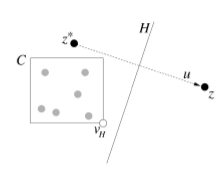
\includegraphics[scale =0.68]{Pruning.png}

\subsection{KMeans++ logic}
In the k-means algorithm, initially we place the k centers randomly before we start the iterations. It needs initial cluster membership of all the data objects to proceed further. The Llyod’s algorithm does not specify the initial placement of centers. There are some cases where we end up placing all the k centers very close to each other. In this case, the algorithm has to perform many iterations before it convergence condition is met or upto the point of maximum iterations mentioned. To solve this problem, the paper[2] provides how to choose the initial k centers. It is based on the intuition to spread out the k centers apart from each other that they be placed in different clusters and hence reducing the number of iterations of the algorithm.The first cluster center is chosen uniformly at random from the data points that are being clustered, after which each subsequent cluster center is chosen from the remaining data points with probability proportional to its distance squared to the point's closest cluster center. In this implementation, we use k-means++ which addresses the second of these obstacles by specifying a procedure to initialize the cluster centers before proceeding with the standard k-means optimization iterations. With the k-means++ initialization, the algorithm is guaranteed to find a solution that is O(log k) competitive to the optimal k-means solution. Basically the kmeans++ reduces the distortion value and finds the good approximation close to the optimal learning.

\subsection{Learning the value of k }
\subsubsection{Gaussian Distribution test}
KMeans algorithm requires users to specify the number of clusters (k). Choosing k becomes difficult when the dimensions of the data increases. It has become an heuristic decision based on some apriori information, performing many trials and assumptions. This paper[] presents a simple algorithm that finds k using a statistical test deciding when to split the k-means center into 2 centers. It uses two hypothesis to decide when to split and when to not. The splitting happens when the data sampled around a center does not follow Gaussian distribution. When the data around a center follows unimodal distribution, then there is no need to split that center as it captures the truth about the subset of the data being surrounded very well. To check this hypothesis, it uses a powerful normality test called Anderson-darling statistic. To simplify the checking, the authors project all the data points onto the vector connecting the two centers that are split thus making it a one-dimensional test. This algorithm takes only one parameter called significance level which is the probability of rejecting the hypothesis that the data around a center follows Gaussian distribution. Empirically, the G-means algorithm works well at finding the correct number of clusters and the locations of genuine cluster centers, and we have shown it works well in moderately high dimensions.
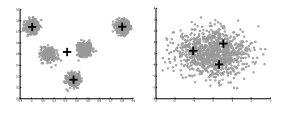
\includegraphics[scale =0.80]{GMeans.png}


\subsubsection{ BIC(Bayesian Information Criterion) scores}
The paper[] also determines the value of k automatically based on the Bayesian Information Criterion scores. It tries so many values of k and scores each clustering model using BIC scores. BIC score is based on the log likelihood of the dataset . It chooses the model with the best BIC score on the data. But the above paper does far better than this BIC method. For example in the 2-d synthetic data with 5 true clusters. This method overfits the data choosing 20 unevenly distributed clusters. 

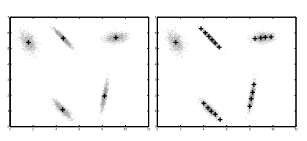
\includegraphics[scale =0.80]{GvsK.png}
 
\section{Implementation}
The algorithm implemented is composed of three modules in addition to the standard kmeans algorithm . The first module to speed up the each step of kmeans iteration using KD trees. The second module is more of preprocessing step for kmeans iterations.It chooses k initial centroids in such a way that they are apart from each other. It helps Kmeans algorithm to converge more fastly.The third module is the algorithm to learn the number of clusters automatically using Gaussian distribution normality test.

\subsection{Module1: Filtering Algorithm }
BBD Tree was constructed from the given set of data. All data are placed into a tree where we choose child nodes by partitioning the data along a plane parallel to the axis of longest radius of bounding box. We maintain for each node, the bounding box of the data stored at that node.  To do a k-means iteration, we need to assign data to clusters and calculate the sum and the number of data assigned to each cluster. This can be done using the below logic:\\ \textit{Pruning:} \begin{itemize}
  \item For each node in the tree, we can rule out some cluster centroids as being too far away from every single point in that bounding box.
  \item If there are more than one center in candidate centers set, then apply filtering recursively.
  \item Once only one center is left in the node, all data in the node can be assigned to that cluster in batch.
\end{itemize}  For each of the k-centers, we need to compute the centroid of the set of data points for which this center is closest. We then move this center to the computed centroid and proceed to the next stage until the convergence condition is met.

\begin{table}[h!]
\centering
\begin{tabular}{ |p{2cm}|p{6cm}|}
 \hline
Algorithm & Implementation\\
 \hline
 \textbf{\textit{KMeans++}}  & standard KMeans algorithm with KMeans++ logic  \\
 \hline
 \textbf{\textit{BBD}}  & standard KMeans algorithm with BBD Trees \\
 \hline
 \textbf{\textit{BBD++}}& standard KMeans algorithm with BBD and KMeans++ logic\\
 \hline
 \textbf{\textit{IBBD++}}& Intelligent KMeans algorithm with BBD and KMeans++ logic that learns k value\\
 \hline
\end{tabular}
\hspace{1mm}
\caption{Variants of Algorithms implemented}
\label{table:1}
\end{table}


\subsection{Module2: KMeans++ seeding}
Initializing of k centroids picked from the data points using careful seeding technique and partitioning the observations into distinct non overlapping groups.\\
The algorithm is as follows:
\begin{enumerate}
  \item Choose one center uniformly at random from among the data points.
  \item For each data point x, compute D(x), the distance between x and the nearest center that has already been chosen.
  \item Choose one new data point at random as a new center, using a weighted probability distribution where a point x is chosen with probability proportional to $D(x)^2$
  \item Repeat Steps 2 and 3 until k centers have been chosen.
\end{enumerate}

\subsection{Module3: Gaussian Test}
I have implemented a wrapper function around the kMeans++ with kdtree to learn the value of k automatically using the algorithm presented in the paper[3]. The only parameter supplied to the algorithm is the significance level of the statistical test $\alpha = 0.001$, which can easily be set in a standard way.The logic behind these algorithm is if the data sampled around a center does not follow gaussian distribution, then split the center into two centers. Otherwise if the data around the center follows gaussian distribution then that center perfectly captures the information of that data. To check the Gaussian Distribution test. We split the center into 2 centers and runs kmeans iterations on that subset of data to adjust the centers to their positions. After this, we calculate the anderson darling static of the data points projected onto the one dimensional vector connecting these two centers.Then Normalize it to N(0,1) cumulative distribution function.
\begin{itemize}
\item If the anderson darling statistic for this data is within the range of critical value 1.8692, then don't split
\item otherwise if it much larger than critical value, then accept split.
\end{itemize}
The G-means algorithm takes linear time and space (plus the cost of the splitting heuristic and test) in the number of data points and dimension, since k-means is itself linear in time and space.


\section{Results}
For evaluating and comparing the implemented algorithms, we are using two indexes namely RandIndex (ri) and AdjustedRandIndex(ari). These are the indexes that measure the quality of clustering
\vspace{1mm}
\newline
\textit{Rand Index}:
Rand list is characterized as the quantity of sets of items that are either in a similar cluster or in various cluster in the two parcels partitioned by the aggregate number of sets of articles. The Rand list lies in the vicinity of 0 and 1. When two partitions agree perfectly, the Rand index achieves the maximum value 1.
\vspace{1mm}
\newline
\textit{AdjustedRandIndex}:An issue with Rand index is that the normal estimation of the Rand index between two arbitrary allotments isn't a steady. This issue is rectified by the Adjusted Rand index that accept the summed up hyper-geometric appropriation as the model of arbitrariness. The Adjusted Rand record has the maximum value 1, and its expected value is 0 on account of irregular clusters. A bigger Adjusted Rand index implies a higher agreement between two allotments. The Adjusted Rand index is suggested for measuring agreement even when the partitions compared have different numbers of clusters.\\


\begin{table}[h!]
\centering
\begin{tabular}{|p{2cm}||p{0.5cm}|p{1.5cm}|p{2cm}||p{1cm}|}
 \hline
Algorithm & K & RandIndex &Adjusted RandIndex & CPU time\\
 \hline
 KMeans++   &64 &  47.14\%   &1.85\% & 2.808s\\
 BBD &64 & 47.09\% & 1.77\% & 1.210s\\
 BBD++ &64 & 47.06\% & 1.68\% & 1.010s\\
 \hline
 KMeans++ & 32 & 48.01\% & 3.24\% & 1.652s\\
 BBD & 32 & 47.01\% & 1.62\% &  1.173s\\
 BBD++ & 32 & 47.08\% & 1.73\% & 1.049s\\
 \hline
 KMeans++ & 4 & 59.55\% & 22.16\% & 0.087s\\
 BBD & 4 & 59.70\% & 22.45\% &  0.151s\\
 BBD++ & 4 & 59.76\% & 22.56\% & 0.209s\\
 \hline
\end{tabular}
\hspace{1mm}
\caption{Results on Multivariate Gaussian Distribution}
\label{table:2}
\end{table}


Four types of Three dimensional Multivaraite gaussian distribution is created with different mu and sigma values with 25000 datapoints allocated to each type. This means that four different clusters were created with 25000 three dimensional data points in each cluster.BBD and Lloyd Algorithm is run on these synthetically created data with different values of k. The two partitions, one is artificially clustered data with 4 clusters, other is the algorithm partitioning on these data is compared with the above mentioned evaluation metrics to check the accuracy of partitioning of the implemented algorithms. The results in the Table \ref{table:1} shows that BBD++ is faster compared to KMeans++ algorithm when the value of k increases and it also outperforms in the both RandIndex and AdjustedRandIndex and minimises the distortion value. 

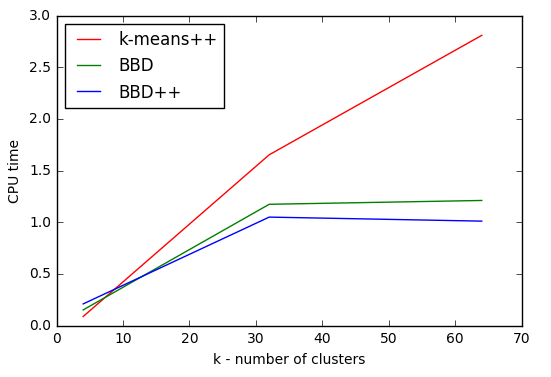
\includegraphics[scale =0.60]{plot.png}

\begin{table}[h!]
\centering
\begin{tabular}{ |p{3cm}|p{2cm}|p{2cm}|}
 \hline
Algorithm & RandIndex &Adjusted RandIndex\\
 \hline
 BBD++ Algorithm &  91.62\%   & 55.80\% \\
 IBBD++ Algorithm & 89.66\% & 45.69\% \\
 \hline
\end{tabular}
\hspace{1mm}
\caption{Training Results on USPS dataset}
\label{table:3}
\end{table}

We were given the cluster labels of the data points in the training data set. The algorithms implemented are run on these training data points and found out the cluster membership of all the data points. These two partitions are evaluated using ri and ari.


\begin{table}[h!]
\centering
\begin{tabular}{ |p{3cm}|p{2cm}|p{2cm}|}
 \hline
Algorithm & RandIndex &Adjusted RandIndex\\
 \hline
BBD++ Algorithm &  90.55\%   & 50.39\% \\
IBBD++ Algorithm &  88.70\% & 40.71\% \\
 \hline
\end{tabular}
\hspace{1mm}
\caption{Testing Results on USPS dataset}
\label{table:4}
\end{table}

For testing USPS dataset, the algorithms takes the data points present in the testing dataset and predicts to which cluster they are nearest to using euclidean distance. In this way, two partitions are evaluated using ri and ari.


\begin{table}[h!]
\centering
\begin{tabular}{ |p{3cm}|p{2cm}|}
 \hline
Algorithm & CPU time\\
 \hline
BBD++ Algorithm &  7.387s \\
IBBD++ Algorithm & 9.989s \\
 \hline
\end{tabular}
\hspace{1mm}
\caption{Time taken for Training and testing on USPS dataset}
\label{table:4}
\end{table}
The extra time taken by IBBD++ algorithm can be attributed to learning the value of k in hierarchial fashion. It starts with k=1 and uses splitting and merging rules according to the normality test. so time taken is O(k) more than the BBD++. we can choose some larger value of k if we have some prior knowledge about the range of k and reduce the time taken by IBBD++


Both the Algorithms BBD++ and IBBD++ was trained and tested on the USPS dataset. Both of them uses KMeans++ logic of initial seed configuration but the latter one does not ask for value of K but rather finds itself using anderson darling statistic. The BBD++ Algorithm gave the best performance with the k = 10 but IBBD++ without any explicit testing for k values it found out itself

The Table \pageref{table:3} shows results of different algorithms with kMeans++ logic of initial seed configuration when run on the US postal services(USPS) dataset.  


\section{Summary and Conclusions}

This paper is the implementation of efficient k-means clustering algorithm using K-dimensional trees along with KMeans++ logic of choosing the proper initial seed configuration of centers before proceeding with standard kMeans iterations.The time taken by the different algorithms has been compared. The results showed that the use of the kmeans++ logic to this efficient implementation using KD trees gives about considerable improvements in the final distortion. Although the initial selection of the centroids in the algorithm takes extra time the k-means part itself converges very fast after this seeding and thus the algorithm actually lowers the computation time too. But KMeans implementation requires user to specify the value of k which becomes especially difficult when the data has many dimensions. So Anderson Darling static is used to learn the value of k without user giving it as a parameter based on a statistical test of subset of the data around a center follows gaussian distribution.This logic is implemented as a wrapper around KMeans++ with KD Trees logic.

The time taken by BBD with the augmented BBD++ is compared with each other. The results have shown that BBD++ does better both in time and in minimising distortion value than the BBD algorithm. Ofcourse, both these algorithms does far better than the Lloyd and KMeans++ algorithm. 

Learning K was added to these algorithms as a wrapper around it and is compared with BBD++ algorithm to check the quality of clustering using randIndex and adjusted RandIndex. Obviously time taken by IBBD++ algorithm is O(K) times more than the BBD++ tree as the algorithm runs every time with increasing value of k in hierarchial fashion. But the quality of clustering is very good on par with other algorithm which knows the value of k on USPS dataset. The above table results shows the closeness of ri and ari of all the algorithms KMeans++, BBD++ and IBBD++. This shows that the all of them perform good clustering of the data points.This is also useful whenever we dont know the value of k and also anything about the information of data




\ifCLASSOPTIONcaptionsoff
  \newpage
\fi




\begin{thebibliography}{1}

\bibitem{IEEEhowto:kopka}
Tapas Kanungo, David M. Mount, Nathan S. Netanyahu, Christine D. Piatko, Ruth Silverman, and Angela Y. Wu \emph{"An Efficient k-Means Clustering Algorithm: Analysis and Implementation. IEEE TRANS. PAMI, 2002" } \hskip 1em plus
  0.5em minus 0.4em\relax 
  \bibitem{IEEEhowto:kopka}
  D. Arthur and S. Vassilvitskii
 \emph{"K-means++: the advantages of careful seeding. ACM-SIAM symposium on Discrete algorithms, 1027-1035, 2007" } \hskip 1em plus
  0.5em minus 0.4em\relax
  \bibitem{IEEEhowto:kopka}
  Anna D. Peterson, Arka P. Ghosh and Ranjan Maitra
 \emph{"A systematic evaluation of different methods for initializing the K-means clustering algorithm. 2010" } \hskip 1em plus
  0.5em minus 0.4em\relax
  \bibitem{IEEEhowto:kopka}
Dan Pelleg and Andrew Moore
\emph{"X-means: Extending K-means with Efficient Estimation of the Number of Clusters. ICML, 2000." } \hskip 1em plus
  0.5em minus 0.4em\relax
  
  \bibitem{IEEEhowto:kopka}
G. Hamerly and C. Elkan. \emph{"Learning the k in k-means. NIPS, 2003" } \hskip 1em plus
  0.5em minus 0.4em\relax
  \bibitem{IEEEhowto:kopka}
Chris Ding, Xiaofeng He, Hongyuan Zha, and Horst Simon.\emph{"Adaptive dimension reduction for clustering high dimensional data. In Proceedings of the 2nd IEEE International Conference on Data Mining, 2002" } \hskip 1em plus
  0.5em minus 0.4em\relax
  \bibitem{IEEEhowto:kopka}
Peter J. Huber. \emph{" Projection pursuit. Annals of Statistics, 13(2):435–475" } \hskip 1em plus
  0.5em minus 0.4em\relax
\bibitem{IEEEhowto:kopka}
K. Alsabti, S. Ranka, and V. Singh. \emph{"An Efficient k-means Clustering Algorithm, Proc. First Workshop High Performance Data Mining, Mar. 2000" } \hskip 1em plus
  0.5em minus 0.4em\relax

\end{thebibliography}



\begin{IEEEbiography}[{\includegraphics[width=1in,height=1.25in,clip,keepaspectratio]{picture}}]{John Doe}
\blindtext
\end{IEEEbiography}


\end{document}


